% Files should be in encoding corresponding to the setting of \usepackage[...]{inputenc}

\documentclass[%      Basic settings of the document
%  draft,    				  % Turn on draft compilation
  12pt,       				% 12 points default font size
	t,                  % The slides should always start at their top (not vertically centered)
	aspectratio=1610,   % Ratio of width and height is 16:10 (corresponding to lecture rooms at Technická 12),
	                    % other options are 43, 149, 169, 54, 32.
	unicode,						% Bookmarks and metainformation in the compiled PDF will be unicode
]{beamer}				    	% Document type 'beamer' is the most often used one for slides
%\usepackage{etex}

\usepackage[utf8]		  %	The input files are in UTF-8 (unicode)
	{inputenc}					% Package for setting input encoding

\usepackage{graphicx} % Package for inclusion of external graphics

\usepackage[
	nohyperlinks				% No hyperlinks to the list of acronyms will be created
]{acronym}						% Package 'acronym' for automated handling of abbreviations and symbols
											% Neccessary for the 'acronym' environment of 'thesis' to work

\usepackage{cmap} 		% This package allows the final PDF
											% is fully "searchable" and "copyable"

%\usepackage{amsmath} %for typesetting advanced mathematics

\usepackage{booktabs} % Package allowing the use of commands \toprule, \midrule, \bottomrule
                      % when creating tables

\usepackage{algorithm2e}	% Package for typesetting algorithms/pseudocode
\usepackage{multirow}
\usepackage{siunitx}  % For decimal alignment

%%%%%%%%%%%%%%%%%%%%%%%%%%%%%%%%%%%%%%%%%%%%%%%%%%%%%%%%%%%%%%%%%
%%%%%%%%                   Definitions                 %%%%%%%%%%
%%%%%%%%%%%%%%%%%%%%%%%%%%%%%%%%%%%%%%%%%%%%%%%%%%%%%%%%%%%%%%%%%

% Variable fields such as your name, title of the thesis atc. are set in this file.
% The file is SHARED between the thesis text and the presentation --- no need to set anything twice.

\usepackage[
  english,			% English study program
%%% Choose one of the thesis types
  %semestral,		%	semestral project (default)
  %bachelor,			%	Bachelor's thesis
  master,			% Master's thesis
  %treatise,			% Treatise on doctoral thesis
  %doctoral,				% Doctoral thesis
%%% Choose one of the options:
%  left,				% Equations and captions will be aligned to the left
  center,			% Equations and captions will be centered (default)
%
  %electronic       % Electronically published version of the thesis; page margins do not alternate with odd- and even-numbered pages
]{thesis}   % Package for typesetting theses


%%% First and last name of the thesis author, following the scheme
% [titles in front]{FirstName}{LastName}[titles after]
% If the author does not have a title in front/after, just delete the entire string '[...]'
\author[Bc.]{Vladislav}{Válek}

%%% Brno University of Technology identification number of author (BUT ID)
\butid{4738967}

%%% First and last name of the advisor
% [titles in front]{FirstName}{LastName}[titles after]
% If the author does not have a title in front/after, just delete the entire string '[...]'
% [titles in front]{FirstName}{LastName}[titles after]
\advisor[Prof. Dr.]{Dirk}{Koch}

%%% First and last name of the opponent
% [titles in front]{FirstName}{LastName}[titles after]
% Makes use only in the presentation for defense;
% in case you do not want the opponent to be shown on the title slide, just comment out the command
% The opponent is not shown in case of the semestral thesis (no opponent exists actually at that time)
% In the case of a doctoral thesis, two to three oponents are typically involved. In such a case, if you want to have them on the title slide, please go to the definition of "VUT title page" in the thesis.sty file, uncomment and adapt their names.
\opponent[Prof. Dr.]{Holger}{Fröning}

%%% Thesis title
%  In the case of a very long thesis title, it may happen that it does not fit
%  into the slot in the footbar of the slides. You may use the command
%  \def\insertshorttitle{Shortened th.\ title}
%  where the shortened version of the title appears as the parameter.
%  If you do not want to shorten the title, you will have to redefine how the slide footbar
%  is generated, see: https://bit.ly/3EJTp5A
\title{Shared CPU-FPGA Filesystem Access on fast NVMe Devices}

%%% Study program/specialization
\specialization{Computer Engineering} %Teleinformatika

%%% Department
%\department{Department of Control and Instrumentation}  %Ústav automatizace a měřicí techniky
%\department{Department of Biomedical Engineering}       %Ústav biomedicínského inženýrství
%\department{Department of Electrical Power Engineering} %Ústav elektroenergetiky
%\department{Department of Electrical and Electronic Technology}   %Ústav elektrotechnologie
%\department{Department of Physics}                      %Ústav fyziky
%\department{Department of Foreign Languages}            %Ústav jazyků
%\department{Department of Mathematics}                  %Ústav matematiky
%\department{Department of Microelectronics}             %Ústav mikroelektroniky
%\department{Department of Radio Electronics}            %Ústav radioelektroniky
%\department{Department of Theoretical and Experimental Electrical Engineering}  %Ústav teoretické a experimentální elektrotechniky
% \department{Department of Telecommunications}           %Ústav telekomunikací
%\department{Department of Power Electrical and Electronic Engineering}   %Ústav výkonové elektrotechniky a elektroniky
\department{Institute of Computer Engineering (ZITI)}

%%% Faculty
%\faculty{Faculty of Architecture}   %Fakulta architektury
% \faculty{Faculty of Electrical Engineering and~Communication}   %Fakulta elektrotechniky a~komunikačních technologií
%\faculty{Faculty of Chemistry}   %Fakulta chemická
%\faculty{Faculty of Information Technology}   %Fakulta informačních technologií
%\faculty{Faculty of Business and Management}   $Fakulta podnikatelská
%\faculty{Faculty of Civil Engineering}   %Fakulta stavební
%\faculty{Faculty of Mechanical Engineering}   %Fakulta strojního inženýrství
%\faculty{Faculty of Fine Arts}   %Fakulta výtvarných umění
\faculty{Faculty of Engineering Sciences}
%
%Logotype selection (in square brackets short logo, in curly brackets full logo):
\facultylogo[logo/FEEC_abbreviation_color_PANTONE_EN]{logo/UTKO_color_PANTONE_EN}


%%% Graduate year (typically the calendar year of the defense)
\graduateyear{2026}
%%% Academic year (typically the year of solution of the thesis in the format n/n+1)
\academicyear{2025/26}
% Date of the defense (makes use only in the presentation slides)
\date{30-March-2026}

%%% Place of the defense
\city{Heidelberg}

%%% Abstract
\abstract{%
This thesis presents an architecture for shared CPU-FPGA filesystem access to NVMe storage using
PCI Express peer-to-peer communication. The goal is to reduce host-memory staging and software
overhead by enabling direct accelerator interaction with an NVMe device while preserving standard
host-side filesystem usage. The implementation combines hardware and software components: an FPGA IP
core (DMA Iuventus) integrated with PCIe endpoint interfaces processes NVMe-related traffic, manages
queue interactions, and issues read/write commands; a userspace software stack based on NDK-SW and
SPDK, together with Linux ublk, provides control-plane integration and exposes a mountable block
device. The complete flow is validated with an exFAT filesystem and demonstrates shared access from
both CPU and FPGA contexts. Experimental evaluation on an AMD Alveo U55C platform with an NVMe SSD
reports resource utilization and request latency for multiple transfer sizes and access patterns. The
results confirm functional operation of the proposed approach and show distinct latency
characteristics for read and write paths, with sublinear read-latency growth for larger transfers.
The work demonstrates practical feasibility of host-bypass storage acceleration and provides a
foundation for future optimization of synchronization, throughput, and multi-device deployment
scenarios.
}

%%% Keywords
\keywrds{%
PCIe, DMA, host-bypassing, peer-to-peer, SPDK, NVMe, FPGA, userspace, ublk, bdev
}

%%% Thanks and acknowledgement
\acknowledgement{%
I would like to thank my supervisor, Prof.\ Dr.\ Dirk Koch for his valuable feedback when writing
this thesis as well as in my research work at the Heidelberg University. I would also like to thank
my colleague, Dr.\ Riadh Ben Abdelhamid, for providing necessary user feedback for the current
course of research. Further, I give many thanks to my colleagues at CESNET, a.l.e., Ing.\ Jakub
Cabal and Ing.\ Martin Špinler, for mentoring me in the development of PCIe-compliant IPs and
software. Finally, I thank my mom, Ing.\ Marta Válková, for supporting me throughout my studies.
}%
      % please go into that file and fill information about you, your topic etc.


%%%%%%%%%%%%%%%%%%%%%%%%%%%%%%%%%%%%%%%%%%%%%%%%%%%%%%%%%%%%%%%%%%%%%%%%
%%%%%   Setting values that appear in the Properties of the PDF  %%%%%%%
%%%%%%%%%%%%%%%%%%%%%%%%%%%%%%%%%%%%%%%%%%%%%%%%%%%%%%%%%%%%%%%%%%%%%%%%
%% If 'hyperref' package is loaded then command '\pdfsettings' can be simply used
\pdfsettings
%  However, you can set the individual fields by hand:
%\hypersetup{
%  pdftitle={Title of the thesis},    	% 'Document Title' field
%  pdfauthor={Author name},   	        % 'Author' field
%  pdfsubject={Type of the document}, 	% 'Subject' field
%  pdfkeywords={Keywords}           	  % 'Keywords' field
%}
\hypersetup{pdfpagemode=FullScreen}  % when opening the file with Adobe Reader,
                                     % automatically open it in fullscreen mode
%%%%%%%%%%%%%%%%%%%%%%%%%%%%%%%%%%%%%%%%%%%%%%%%%%%%%%%%%%%%%%%%%%%%%%%

\usetheme{VUT} 				% colours and layout corresponding to the BUT style
% alternatively, other styles can be used, such as
%\usetheme{Darmstadt} \usecolortheme{default2}
% but with no guarantees
\logoheader					% inserts small BUT FEEC logotype in the header; leave this in use

\setbeamertemplate{caption}[default]

\begin{document}

% if you do not use the following command, the lower right corner of each slide will contain active navigation symbols
\disablenavigationsymbols

% the title slide will be created without header, footer etc.
\maketitle

%%%%%%%%%%%%%%%%%%%%%%%%%%%%%%%%%%%%%%%%%%%%%%%%%%%%%%%%%%%%%%%%%%%%%%%%%%%%%%%%%%%%%%%%%%%
\begin{frame}
	\frametitle{Content}
	\begin{itemize}
			\item Motivation and goals
			\item PCI Express and NVMe essentials
			\item Hardware architecture
			\item Shared filesystem access
			\item Evaluation highlights
			\item Demo
			\item Conclusion
	\end{itemize}
\end{frame}

%%%%%%%%%%%%%%%%%%%%%%%%%%%%%%%%%%%%%%%%%%%%%%%%%%%%%%%%%%%%%%%%%%%%%%%%%%%%%%%%%%%%%%%%%%%
\begin{frame}
	\frametitle{Motivation}
	\begin{itemize}
		\item Conventional CPU-facilitated workflow introduces an overhead
		\item Host memory used for staging (double copying)
		\item Direct access to NVMe storage from accelerator
		\item Standardized filesystem
	\end{itemize}

	\vspace{0.4cm}
	\textbf{Goal of this work:} enable shared CPU-FPGA filesystem access to NVMe while preserving a standard Linux workflow.
\end{frame}

%%%%%%%%%%%%%%%%%%%%%%%%%%%%%%%%%%%%%%%%%%%%%%%%%%%%%%%%%%%%%%%%%%%%%%%%%%%%%%%%%%%%%%%%%%%

\begin{frame}
	\frametitle{PCI Express}

	\begin{columns}[T] 					% columns environment, top placement
		\begin{column}{0.6\textwidth}	% first column
			\begin{itemize}
				\item Since 2003
				\item Streaming \& memory-mapped
				\item Serial-parallel hybrid
				\item Specification -- Gen7 (242~GBps)
				\item Devices -- Gen5 (63.015~GBps)
				\item Support on FPGAs
			\end{itemize}

			\centering
			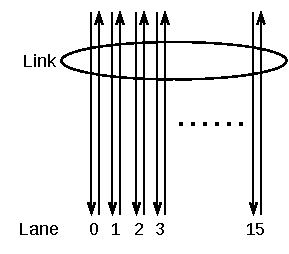
\includegraphics[scale=0.9]{pict/pcie_link_schema.pdf}
		\end{column}
		%
		\begin{column}{0.4\textwidth}		% second column
			\centering
			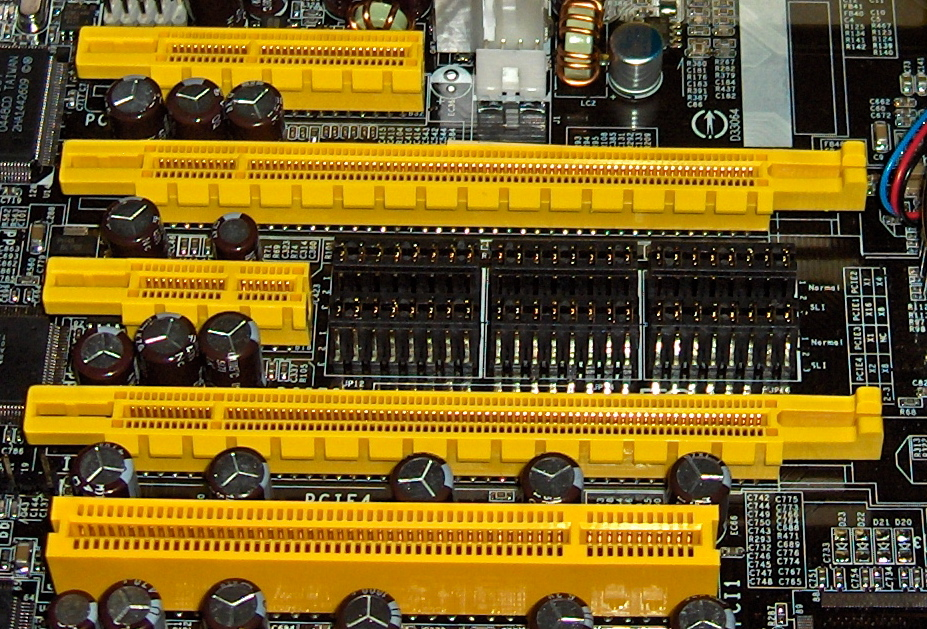
\includegraphics[width=\columnwidth]{pict/cem_conns.jpg}
			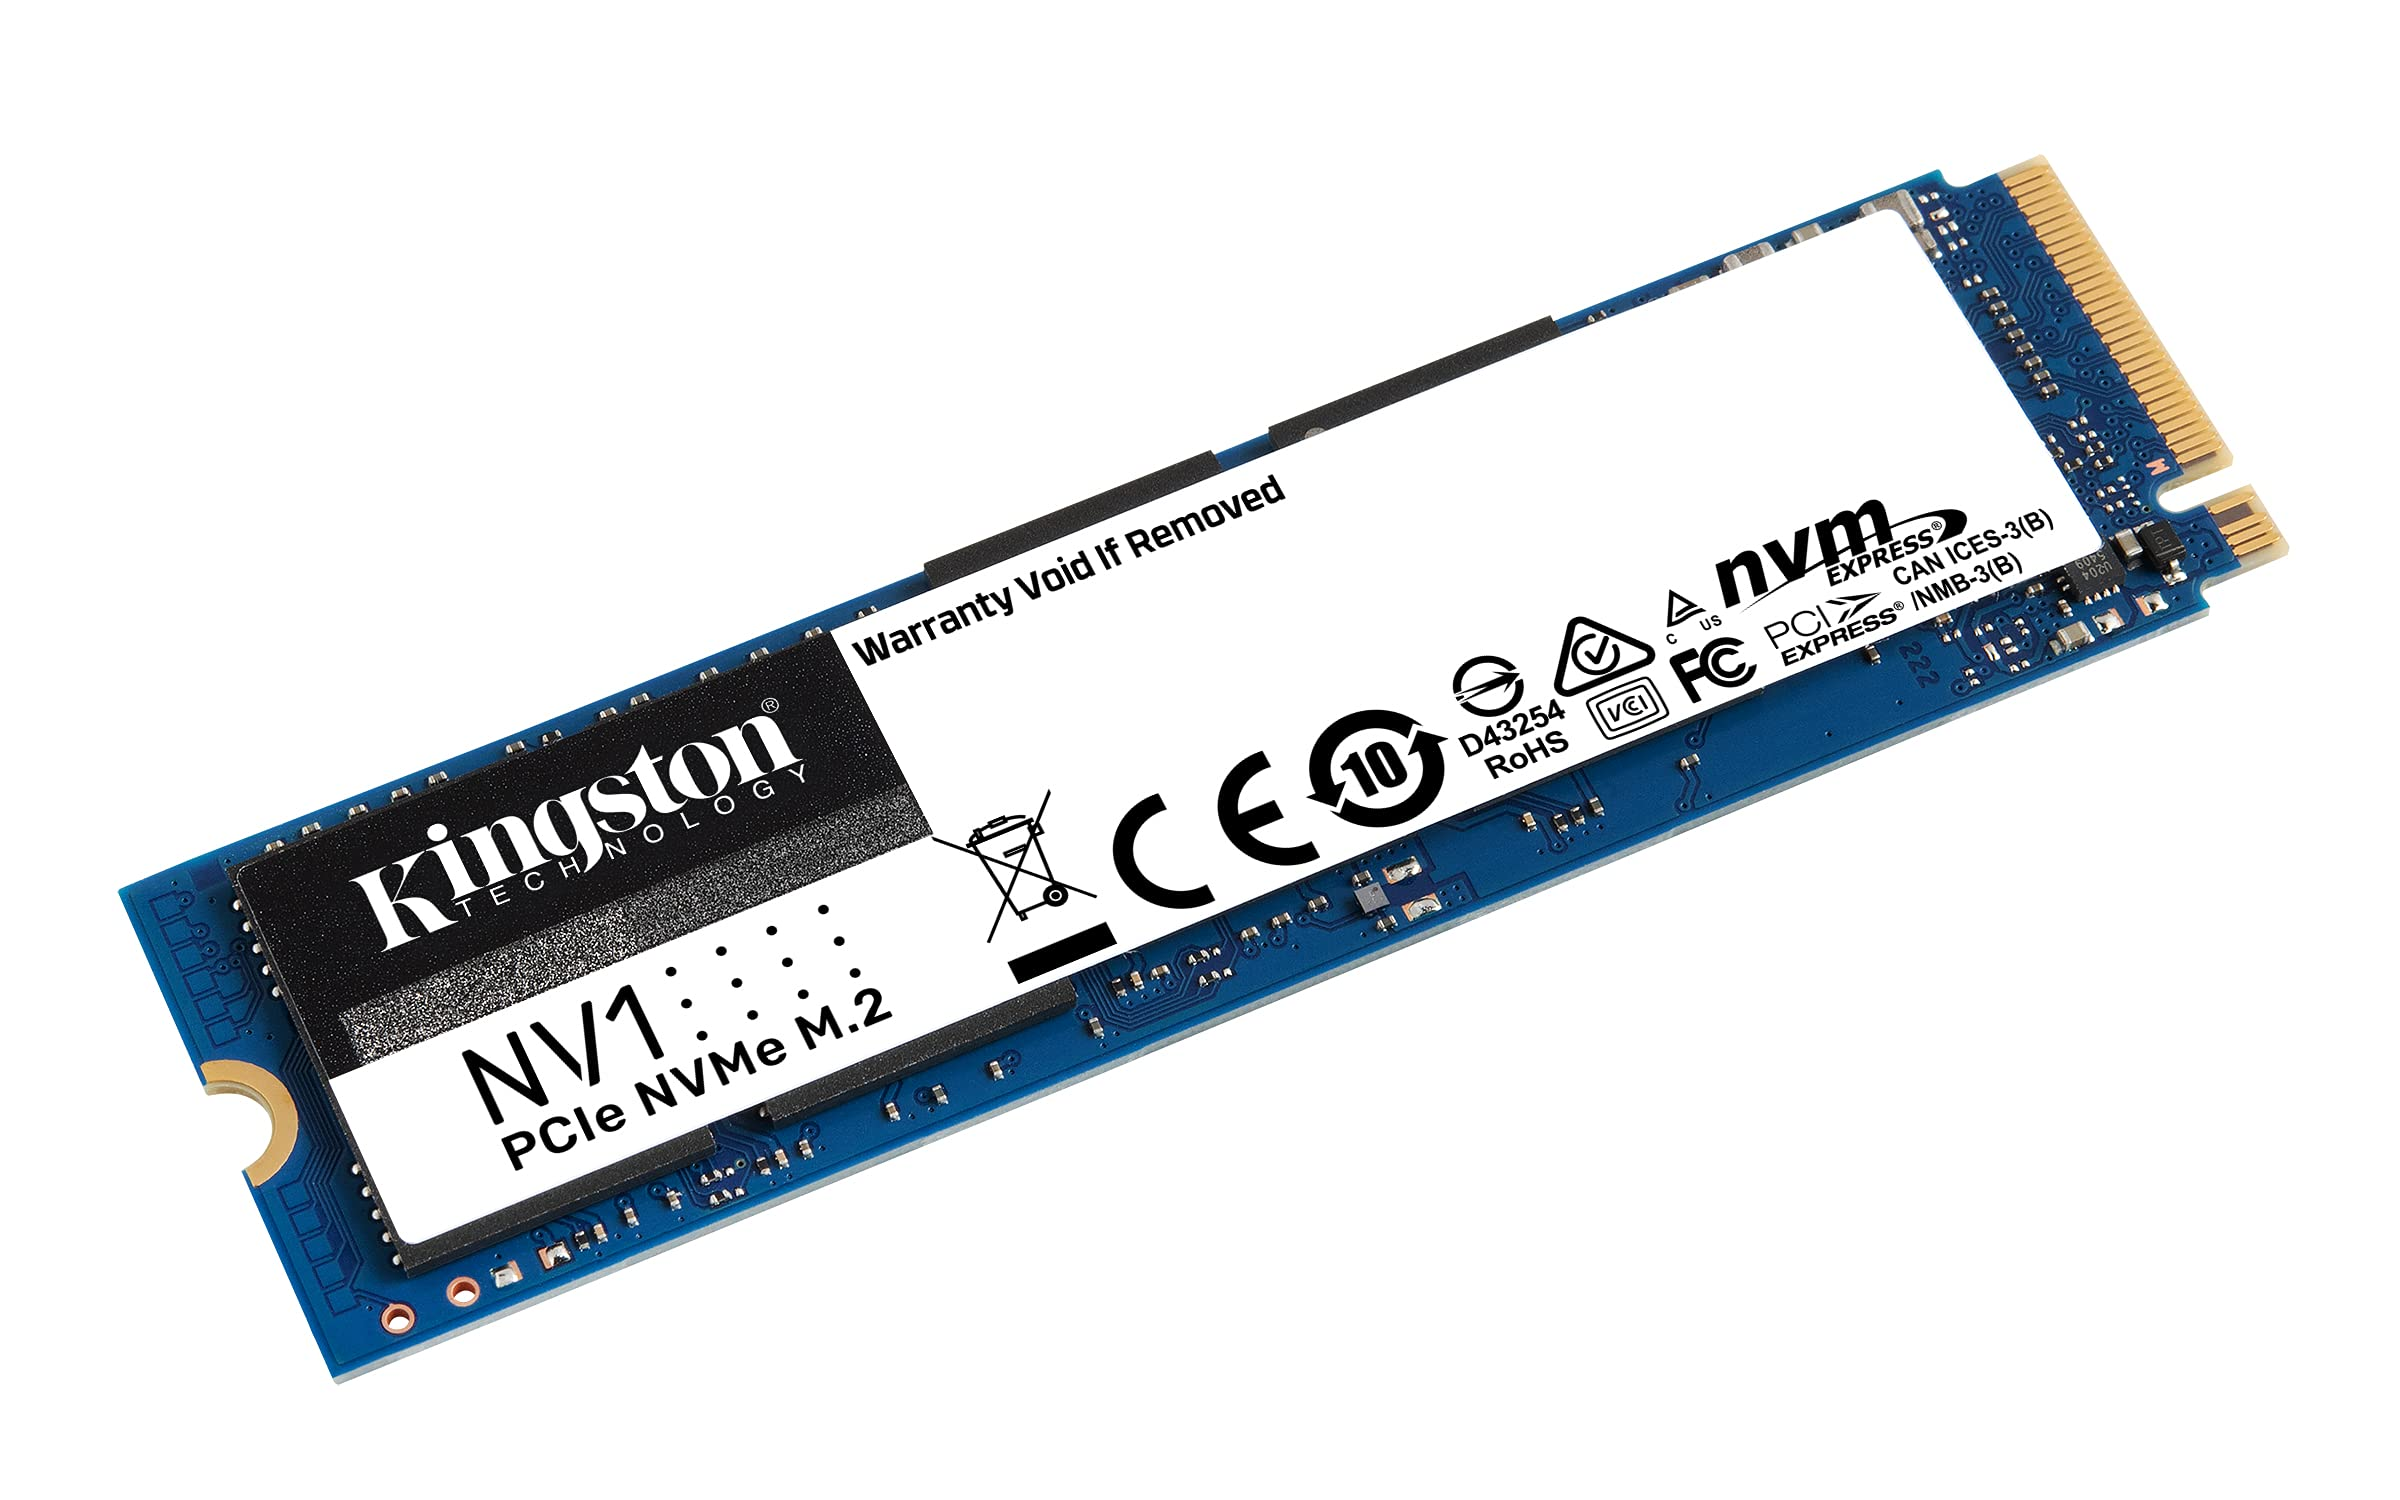
\includegraphics[width=\columnwidth]{pict/nvme_drive.jpg}
		\end{column}
	\end{columns}											% end of the main environment
\end{frame}

%%%%%%%%%%%%%%%%%%%%%%%%%%%%%%%%%%%%%%%%%%%%%%%%%%%%%%%%%%%%%%%%%%%%%%%%%%%%%%%%%%%%%%%%%%%
		% \begin{figure}%
		% 	\centering
		% 	\vspace{1cm}	              % horizontal space
		% 	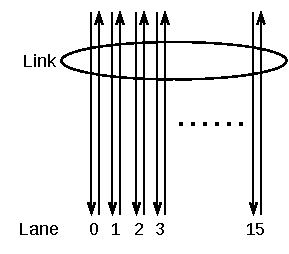
\includegraphics[scale=0.9]{pict/pcie_link_schema.pdf}
		% \end{figure}

\begin{frame}
	\frametitle{PCIe Interconnect}
	\begin{columns}[T] 					% columns environment, top placement
		\begin{column}{0.5\textwidth}	% first column
			\begin{itemize}
				\item Switched point-to-point interconnect
				\item Tree topology
				\item Root Complex, Switches, Endpoints
				\item Address-based routing*
				\item Peer-to-peer transport (host bypassing)
				\item Transaction Layer Packet (TLP)
					\begin{itemize}
						\item Memory Write request
						\item Memory Read request
						\item Completion
					\end{itemize}
			\end{itemize}
			% \vspace{0.1cm}
			\centering
			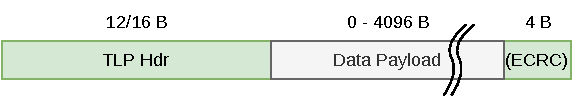
\includegraphics[width=1.2\columnwidth]{pict/data_units-tlp.pdf}
		\end{column}
		%
		\begin{column}{0.5\textwidth}		% second column
			\vspace{1cm}
			\centering
			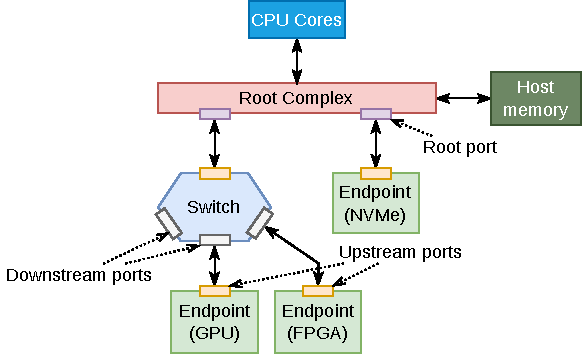
\includegraphics[width=1.05\columnwidth]{pict/host_topology-raw_topology.pdf}
		\end{column}
	\end{columns}											% end of the main environment
\end{frame}

%%%%%%%%%%%%%%%%%%%%%%%%%%%%%%%%%%%%%%%%%%%%%%%%%%%%%%%%%%%%%%%%%%%%%%%%%%%%%%%%%%%%%%%%%%%
\begin{frame}
	\vspace{1cm}
	\begin{columns}[T] 					% columns environment, top placement
		\begin{column}{0.55\textwidth}	% first column
			\begin{figure}%
				\centering
				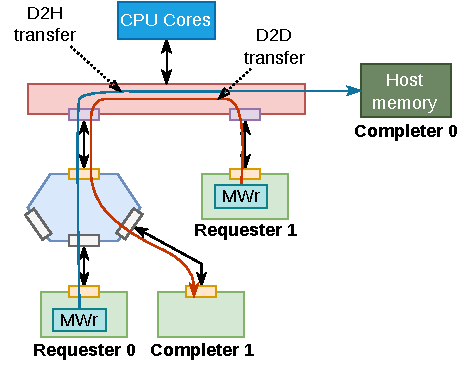
\includegraphics[width=\columnwidth]{pict/host_topology-d2d_write.pdf}
				\caption{Write request path}
			\end{figure}
		\end{column}
		%
		\begin{column}{0.45\textwidth}		% second column
			\begin{figure}%
				\centering
				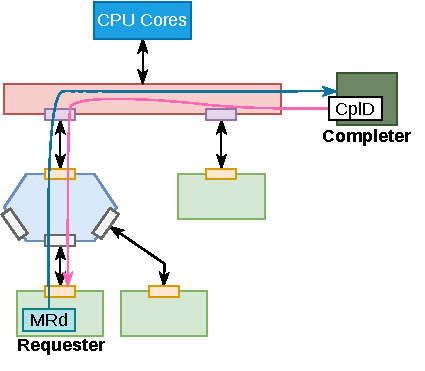
\includegraphics[width=\columnwidth]{pict/host_topology-simple_read.pdf}
				\caption{Read request path}
			\end{figure}
		\end{column}
	\end{columns}											% end of the main environment
\end{frame}

%%%%%%%%%%%%%%%%%%%%%%%%%%%%%%%%%%%%%%%%%%%%%%%%%%%%%%%%%%%%%%%%%%%%%%%%%%%%%%%%%%%%%%%%%%%
\begin{frame}
	\frametitle{Configuration}
	\begin{columns}[T] 					% columns environment, top placement
		\begin{column}{0.4\textwidth}	% first column
			\begin{itemize}
				\item Configured on startup
				\item Bus Mastering
				\item Base Address Register (BAR)
				\item Enable memory-mapped IO
			\end{itemize}
		\end{column}
		%
		\begin{column}{0.6\textwidth}		% second column
			\centering
			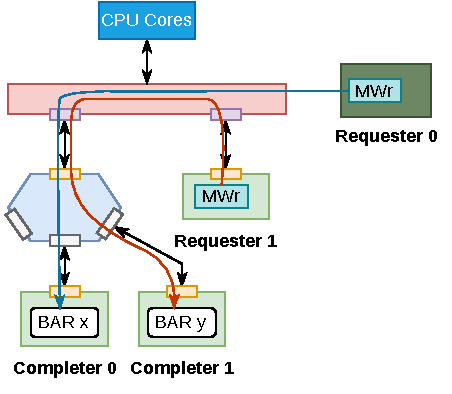
\includegraphics[width=\columnwidth]{pict/host_topology-with_bars.pdf}
		\end{column}
	\end{columns}											% end of the main environment
\end{frame}

%%%%%%%%%%%%%%%%%%%%%%%%%%%%%%%%%%%%%%%%%%%%%%%%%%%%%%%%%%%%%%%%%%%%%%%%%%%%%%%%%%%%%%%%%%%
\begin{frame}
	\frametitle{Non-volatile Memory Express (NVMe)}
	\begin{columns}[T] 					% columns environment, top placement
		\begin{column}{0.5\textwidth}	% first column
			\begin{itemize}
				\item Command based
				\item Queue-pair model: submission and completion queues
				\item Up to $2^{16}$ queues
				\item Up to $2^{16}$ commands
				\item Pointers to synchronize queue state (doorbells)
				\item Namespace divided to sectors
				\item Logical Block Address (LBA)
			\end{itemize}
		\end{column}
		%
		\begin{column}{0.5\textwidth}		% second column
			\centering
			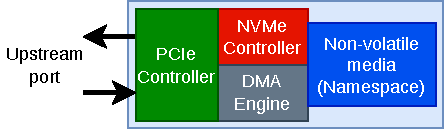
\includegraphics[width=\columnwidth]{pict/ziti_easy_arch-nvme_design.pdf}

			\vspace{0.5cm}
			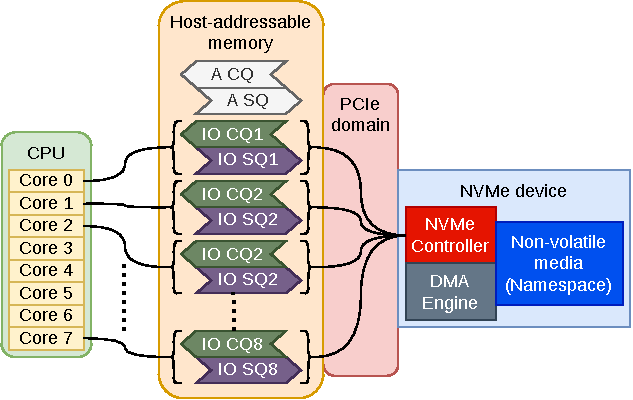
\includegraphics[width=\columnwidth]{pict/ziti_easy_arch-nvme_initialized_system.pdf}
		\end{column}
	\end{columns}											% end of the main environment
\end{frame}

%%%%%%%%%%%%%%%%%%%%%%%%%%%%%%%%%%%%%%%%%%%%%%%%%%%%%%%%%%%%%%%%%%%%%%%%%%%%%%%%%%%%%%%%%%%
\begin{frame}
	\frametitle{Read command}
	\centering
	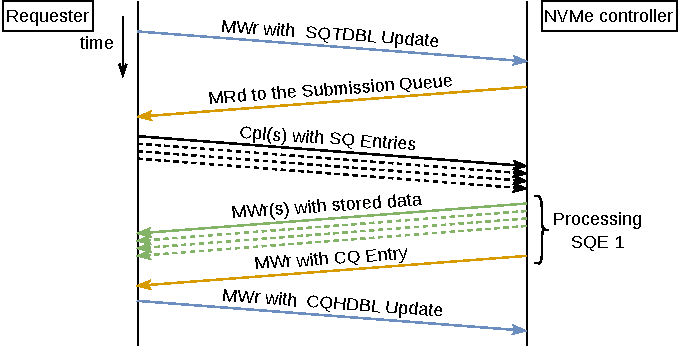
\includegraphics[width=\textwidth]{pict/nvme_prot-read_one.pdf}
\end{frame}

%%%%%%%%%%%%%%%%%%%%%%%%%%%%%%%%%%%%%%%%%%%%%%%%%%%%%%%%%%%%%%%%%%%%%%%%%%%%%%%%%%%%%%%%%%%
\begin{frame}
	\frametitle{Write command}
	\centering
	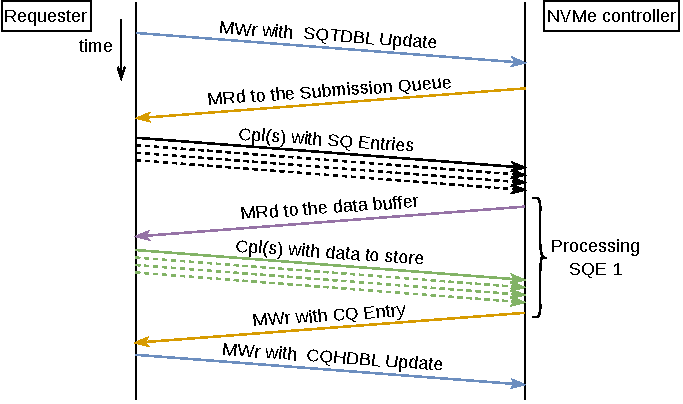
\includegraphics[width=0.95\textwidth]{pict/nvme_prot-write_one.pdf}
\end{frame}

%%%%%%%%%%%%%%%%%%%%%%%%%%%%%%%%%%%%%%%%%%%%%%%%%%%%%%%%%%%%%%%%%%%%%%%%%%%%%%%%%%%%%%%%%%%
\begin{frame}
	\frametitle{Hardware implementation}
	\begin{columns}[T] 					% columns environment, top placement
		\begin{column}{0.5\textwidth}	% first column
			\begin{itemize}
				\item FPGA card: AMD Alveo U55C
				\item Up to PCIe Gen4x16
				\item Accelerator BARs hold queues and data buffers
				\item DMA Iuventus IP
				\item Interface to user logic
				\item Maximum IO size of 256 LBAs
			\end{itemize}
		\end{column}
		%
		\begin{column}{0.5\textwidth}		% second column
			% \vspace{1cm}
			\centering
			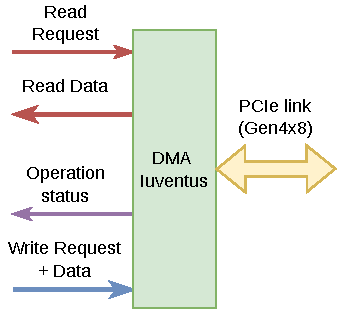
\includegraphics[width=\columnwidth]{pict/dma_iuventus_scheme-simple_arch.pdf}
		\end{column}
	\end{columns}											% end of the main environment
\end{frame}

\begin{frame}
	\centering
	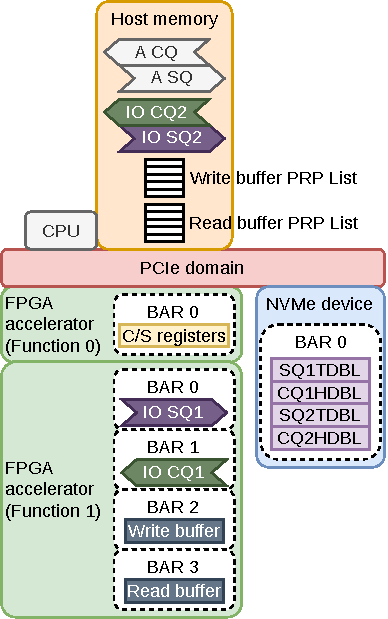
\includegraphics[height=0.95\textheight]{pict/ziti_easy_arch-iuventus_memory_scheme.pdf}
\end{frame}

%%%%%%%%%%%%%%%%%%%%%%%%%%%%%%%%%%%%%%%%%%%%%%%%%%%%%%%%%%%%%%%%%%%%%%%%%%%%%%%%%%%%%%%%%%%
\begin{frame}
	\frametitle{Userspace drivers}
	\begin{columns}[T] 					% columns environment, top placement
		\begin{column}{0.5\textwidth}	% first column
			\begin{itemize}
				\item System calls are expensive
				\item Kernel development difficult
				\item More libraries
				\item Easier debugging
				\item Storage Performance Development Kit (SPDK)
				\item Poll mode driver (PMD)
				\item No interrupts
				\item Lower latency, higher throughput
			\end{itemize}
		\end{column}
		%
		\begin{column}{0.5\textwidth}		% second column
			\vspace{1cm}
			\centering
			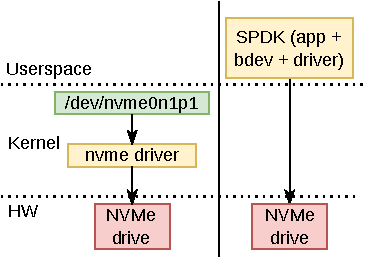
\includegraphics[width=\columnwidth]{pict/ublk-driver_type.pdf}
		\end{column}
	\end{columns}											% end of the main environment
\end{frame}

%%%%%%%%%%%%%%%%%%%%%%%%%%%%%%%%%%%%%%%%%%%%%%%%%%%%%%%%%%%%%%%%%%%%%%%%%%%%%%%%%%%%%%%%%%%
\begin{frame}
	\frametitle{Filesystem}
	\begin{columns}[T]
		\begin{column}{0.4\textwidth}
			\begin{itemize}
				\item Everything in kernel
				\item Block vs.\ character devices
				\item Only bdevs run filesystem
			\end{itemize}
		\end{column}
		%
		\begin{column}{0.6\textwidth}
			% \vspace{1cm}
			\centering
			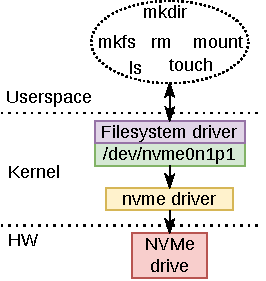
\includegraphics[width=0.8\columnwidth]{pict/ublk-normal_filesystem.pdf}
		\end{column}
	\end{columns}
\end{frame}

%%%%%%%%%%%%%%%%%%%%%%%%%%%%%%%%%%%%%%%%%%%%%%%%%%%%%%%%%%%%%%%%%%%%%%%%%%%%%%%%%%%%%%%%%%%
\begin{frame}
	\frametitle{Shared CPU-FPGA filesystem}
	\begin{columns}[T] 					% columns environment, top placement
		\begin{column}{0.4\textwidth}	% first column
			\begin{enumerate}
				\item Keep userspace drivers
				\item Create block device
				\item Publish bdev to the kernel
				\item Initialize filesystem (exFAT)
				\item Mount filesystem
				\item Forward IO requests to the ublk server
			\end{enumerate}
		\end{column}
		%
		\begin{column}{0.6\textwidth}		% second column
			\vspace{0.5cm}
			\centering
			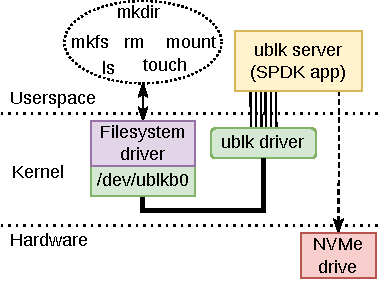
\includegraphics[width=\columnwidth]{pict/ublk-app.pdf}
		\end{column}
	\end{columns}											% end of the main environment
\end{frame}

%%%%%%%%%%%%%%%%%%%%%%%%%%%%%%%%%%%%%%%%%%%%%%%%%%%%%%%%%%%%%%%%%%%%%%%%%%%%%%%%%%%%%%%%%%%
\begin{frame}
	\frametitle{Evaluation: Resource utilization}
	\begin{table}[!ht]
		\centering
		\caption{FPGA resource consumption after design implementation phase (fully placed and routed)}
		% \label{tab:res_cons}
		\begin{tabular}{lcccc|cc}
		\toprule
		\multirow{2}{*}{\textbf{Resource type}} & \multicolumn{2}{c}{\textbf{DMA Iuventus}} &
		\multicolumn{2}{c}{\textbf{PCIe IP}} & \multicolumn{2}{c}{\textbf{Test design total}} \\
		\cmidrule(lr){2-3}\cmidrule(lr){4-5}\cmidrule(lr){6-7}
						& \textbf{abs} & \textbf{\%} & \textbf{abs} & \textbf{\%} &
						\textbf{abs} & \textbf{\%} \\
		\midrule
		LUT             & 12532  & 0.96      & 9155   & 0.70      & 24792  & 1.90  \\
		LUTRAM          & 268    & 0.04      & 1148   & 0.19      & 1938   & 0.32  \\
		FF              & 22208  & 0.85      & 24903  & 0.96      & 52498  & 2.01  \\
		BRAM Tile       & 134.5  & 6.67      & 30.5   & 1.51      & 194.5  & 9.65  \\
		URAM            & 0      & 0         & 0      & 0         & 11     & 1.15  \\
		\bottomrule
		\end{tabular}
	\end{table}
\end{frame}

%%%%%%%%%%%%%%%%%%%%%%%%%%%%%%%%%%%%%%%%%%%%%%%%%%%%%%%%%%%%%%%%%%%%%%%%%%%%%%%%%%%%%%%%%%%
\begin{frame}
	\frametitle{Evaluation: Byte and IO throughput}
	\begin{itemize}
		\item Measured over period of $2^{28}$ cycles (\textasciitilde1 second)
	\end{itemize}
\end{frame}

%%%%%%%%%%%%%%%%%%%%%%%%%%%%%%%%%%%%%%%%%%%%%%%%%%%%%%%%%%%%%%%%%%%%%%%%%%%%%%%%%%%%%%%%%%%
\begin{frame}
	\centering
	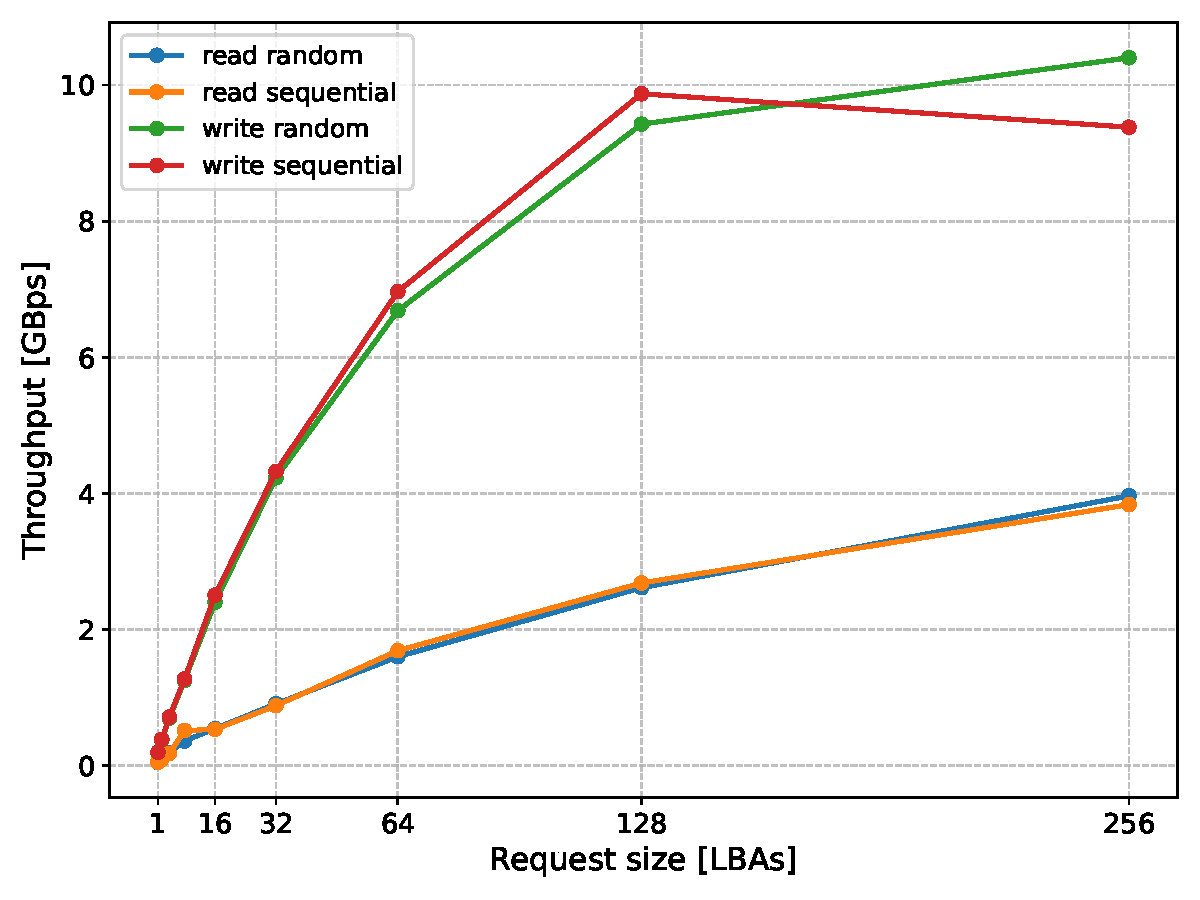
\includegraphics[width=0.9\textwidth]{pict/throughput_all_modes.pdf}
\end{frame}

%%%%%%%%%%%%%%%%%%%%%%%%%%%%%%%%%%%%%%%%%%%%%%%%%%%%%%%%%%%%%%%%%%%%%%%%%%%%%%%%%%%%%%%%%%%
\begin{frame}
	\centering
	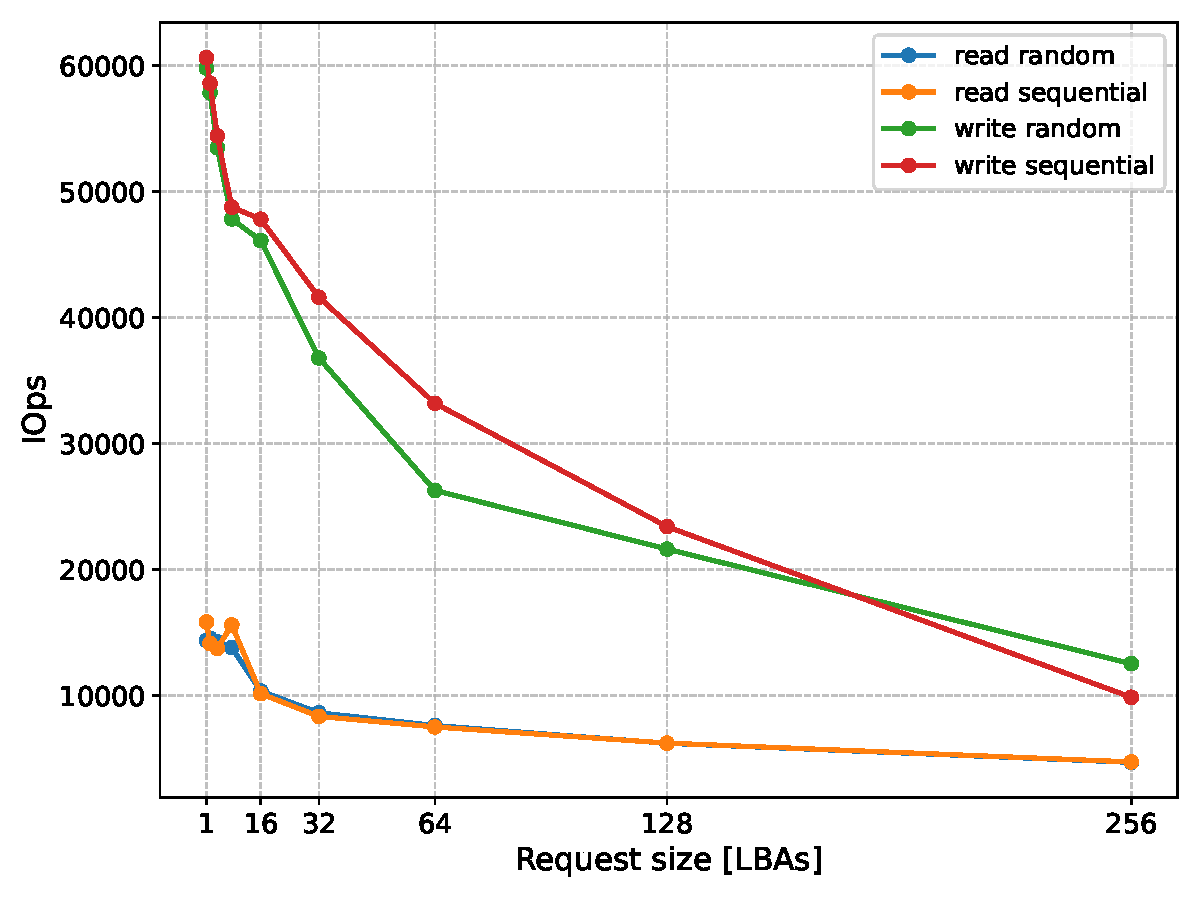
\includegraphics[width=0.9\textwidth]{pict/iops_all_modes.pdf}
\end{frame}

%%%%%%%%%%%%%%%%%%%%%%%%%%%%%%%%%%%%%%%%%%%%%%%%%%%%%%%%%%%%%%%%%%%%%%%%%%%%%%%%%%%%%%%%%%%
\begin{frame}
	\frametitle{Evaluation: Latency}
	\begin{itemize}
		\item Timestamp width 28 bits (\textasciitilde1 second delay)
		\item Results stored in histogram (1 bin = 512 ns)
		\item 50000 repetitions
	\end{itemize}

	% \begin{table}[!ht]
		\centering
		% \setlength{\tabcolsep}{4pt}
		% \caption[Latency measurement results]{Results of latency measurement for different operations,
		% request sizes and access pattern (\si{\micro\second})}
		% \label{tab:latency-results}
		\begin{tabular}{lllSSSSS@{}}
			\toprule
			\textbf{Op.} & \textbf{Access} & \textbf{Size} & {\textbf{Min}} &
			{\boldmath $P_{50}$} &  {\boldmath $P_{99}$} & {\textbf{Max}} \\
			& & {[LBAs]} & & & & & \\
			\midrule
			RD  & Random     &   1 &  46.64 &  66.71 &    81.75 & 1952.72 \\
				&            & 256 & 143.27 & 203.46 &  238.26 & 357.50 \\
			\addlinespace
				& Sequential &   1 &  62.12 &  63.15 &   65.97 & 173.30 \\
				&            & 256 & 144.12 & 201.50 &  237.61 & 1904.40 \\
			\midrule
			WR  & Random     &   1 &   8.34 &    8.61 &   107.28 & 5379.27 \\
				&            & 256 &  54.05 &   62.65 &   454.14 & 6692.82 \\
			\addlinespace
				& Sequential &   1 &   8.34 &     8.45 &     8.70 &  10.19 \\
				&            & 256 &  54.10 &   71.57 &   251.26 & 5860.76 \\
			\bottomrule
		\end{tabular}
	% \end{table}

\end{frame}


%%%%%%%%%%%%%%%%%%%%%%%%%%%%%%%%%%%%%%%%%%%%%%%%%%%%%%%%%%%%%%%%%%%%%%%%%%%%%%%%%%%%%%%%%%%
\begin{frame}[c]
	\begin{block}{Demo}
		Shared read/write filesystem access.
	\end{block}
\end{frame}

%%%%%%%%%%%%%%%%%%%%%%%%%%%%%%%%%%%%%%%%%%%%%%%%%%%%%%%%%%%%%%%%%%%%%%%%%%%%%%%%%%%%%%%%%%%
\begin{frame}
	\frametitle{Conclusion}
	\begin{itemize}
		\item PCIe peer-to-peer path avoids host-memory staging
		\item Linux filesystem access is maintained
		\item Design verified using functional verification (CocoTB)
		\item Validated in hardware
		\item Shared CPU-FPGA filesystem access to NVMe is operational
		\item Future development
			\begin{itemize}
				\item More outstanding commands
				\item Support for more NVMe drives
				\item Alveo V80 support
				\item Support for both NVMe and host memory transfers
			\end{itemize}
	\end{itemize}
\end{frame}

%%%%%%%%%%%%%%%%%%%%%%%%%%%%%%%%%%%%%%%%%%%%%%%%%%%%%%%%%%%%%%%%%%%%%%%%%%%%%%%%%%%%%%%%%%%
\begin{frame}[c]
	\begin{center}
		{\Huge Thank you for your attention!}

		\vspace{1cm}	              % horizontal space
		{\Large Any questions?}
	\end{center}
\end{frame}

%%%%%%%%%%%%%%%%%%%%%%%%%%%%%%%%%%%%%%%%%%%%%%%%%%%%%%%%%%%%%%%%%%%%%%%%%%%%%%%%%%%%%%%%%%%
\begin{frame}[noframenumbering]
	\frametitle{DMA Iuventus architecture}
	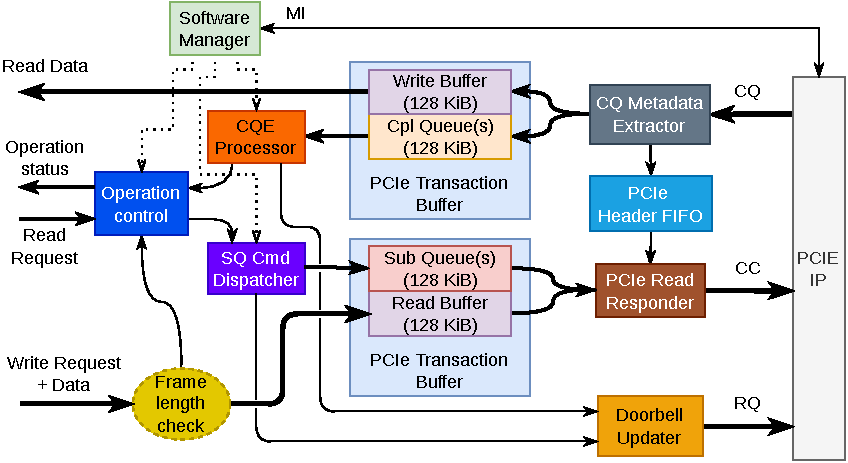
\includegraphics[width=\textwidth]{pict/dma_iuventus_scheme.pdf}
\end{frame}
\end{document}

% \begin{frame}
% 	\frametitle{Key Tools}

% 	% environment 'alertblock' for alerting the particular info
% 	\begin{alertblock}{The key tool in this thesis is the Euler formula}
% 		$$\eul^{\jmag x}=\cos x + \jmag\sin x$$
% 	\end{alertblock}

% 	\vspace{4ex}
% 	The Euler identity is the special case of the above, with $x=\uppi$\,:

% 	% environment 'block'
% 	\begin{block}{Euler identity}
% 		$$\eul^{\jmag \uppi}=\cos \uppi + \jmag\sin \uppi,$$\\
% 		from which it follows that
% 		$$\eul^{\jmag \uppi}+1=0.$$
% 	\end{block}
% \end{frame}


%%%%%%%%%%%%%
% \begin{frame}
% 	\frametitle{Printed Circuit Board}

% 	\begin{columns}[T] 								% columns environment, top placement
% 		\begin{column}{0.4\textwidth}		% first column
% 			Depicted model contains:\\[2ex]
% 			%
% 			\begin{itemize}
% 				\item Board
% 				\item Signals
% 				\item Battery
% 			\end{itemize}
% 		\end{column}
% 		%
% 		\begin{column}{0.6\textwidth}		% second column
% 			\begin{figure}%
% 				\centering
% 				\vspace{1cm}	              % horizontal space
% 				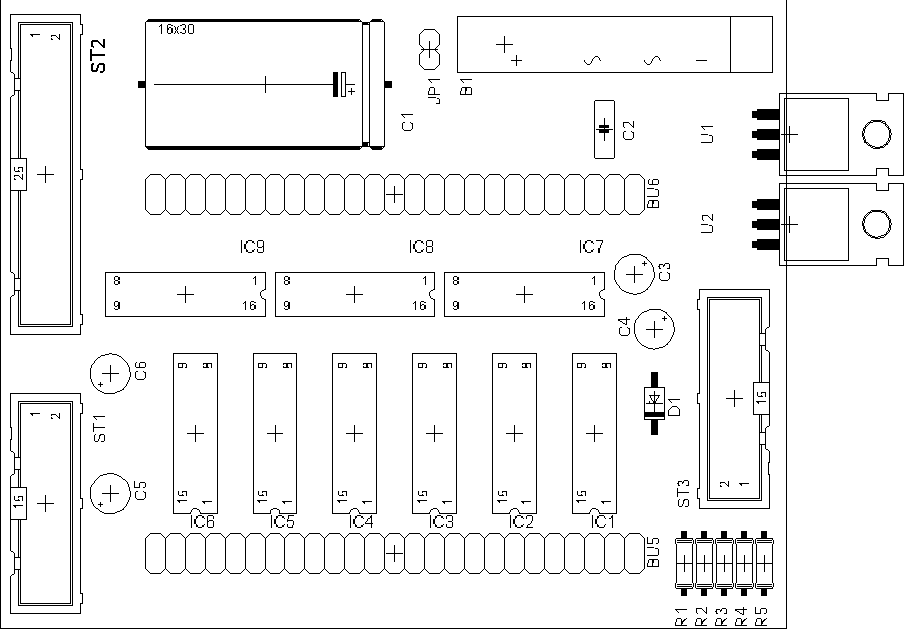
\includegraphics[width=0.8\columnwidth]{pict/soucastky}
% 			\end{figure}
% 		\end{column}
% 	\end{columns}											% end of the main environment
% \end{frame}


%%%%%%%%%%%%%
% \begin{frame}
% 	\frametitle{Results}
% 	\vspace{1cm}
% 	\begin{table}[]
% 		\centering
% 		\caption{Results of measurement in mobile networks}
% 		\label{tab:table.results}
% 			\begin{tabular}{lcc}
% 				\toprule
% 					Technology  & Speed, download [kB/s] & Speed, upload [kB/s] \\
% 				\midrule
% 					GPRS (2,5G)	& 7,2 	& 3,6\\
% 					UMTS 3G     & 48 		& 48\\
% 					HSPA (3,5G)	&	1\,706	&	720\\
% 					LTE (4G) 		& 40\,750 & 10\,750\\
% 				\bottomrule
% 			\end{tabular}
% 	\end{table}
% \end{frame}


% opponent's questions
% \frame{
% \frametitle{Questions of the Opponent}
% 	\emph{Is there some relationship between your formula (1.2) and integral Maxwell equations?}\\[2ex]
% 	%
% 	Well, yes, it might be\,\dots
% }
